\documentclass[../manuale-utente.tex]{subfiles}

\begin{document}

\subsection{Requisiti}%
\label{sub:mobile_app_requisiti}

\begin{description}
    \item[Sistema operativo:] Android 5.0 o superiore.
    \item[Geolocalizzazione:] A-GPS obbligatorio, GLONASS e Galileo consigliati.
    \item[Sensori consigliati:] Giroscopio, Accelerometro.
\end{description}

\subsection{Installazione}%
\label{sub:mobile_app_installazione}

Attualmente \textit{Stalker} non è disponibile per il download tramite \textit{\glossarioLocale{Play Store}}, ma è disponibile solo tramite installazione manuale.
Per installare \textit{Stalker} è necessario:
\begin{itemize}
    % dire esplicitamente qual è il link per installare Stalker
    \item Scaricare l'\textit{\glossarioLocale{APK}} di \textit{Stalker} dall'apposito link dal browser del vostro smartphone.
    \item Accedere ad un \glossarioLocale{file manager}.
    \item Accedere alla cartella download dello smartphone.
    \item Selezionare l'applicazione di \textit{Stalker} appena scaricata.
    \item Se richiesto, attivare l'impostazione per la privacy \textit{Origini sconosciute} (consultare la sotto-sezione §~\ref{subs:mobile_app_attivare_sorgenti_sconosciute}).
    \item Avviare la procedura di installazione.
    \item Fornire i permessi richiesti dalla mobile application.
\end{itemize}
Nel caso ci fossero problemi durante l'installazione di \textit{Stalker}, vi preghiamo di consultare la sotto-sezione §~\ref{subs:mobile_app_risoluzione_problemi}.

\subsection{Manuale d'uso}%
\label{sub:manuale_uso_mobile}

\subsubsection{Pagina di accesso}%
\label{subs:pagina_di_accesso}

\begin{figure}[H]
    \centering
    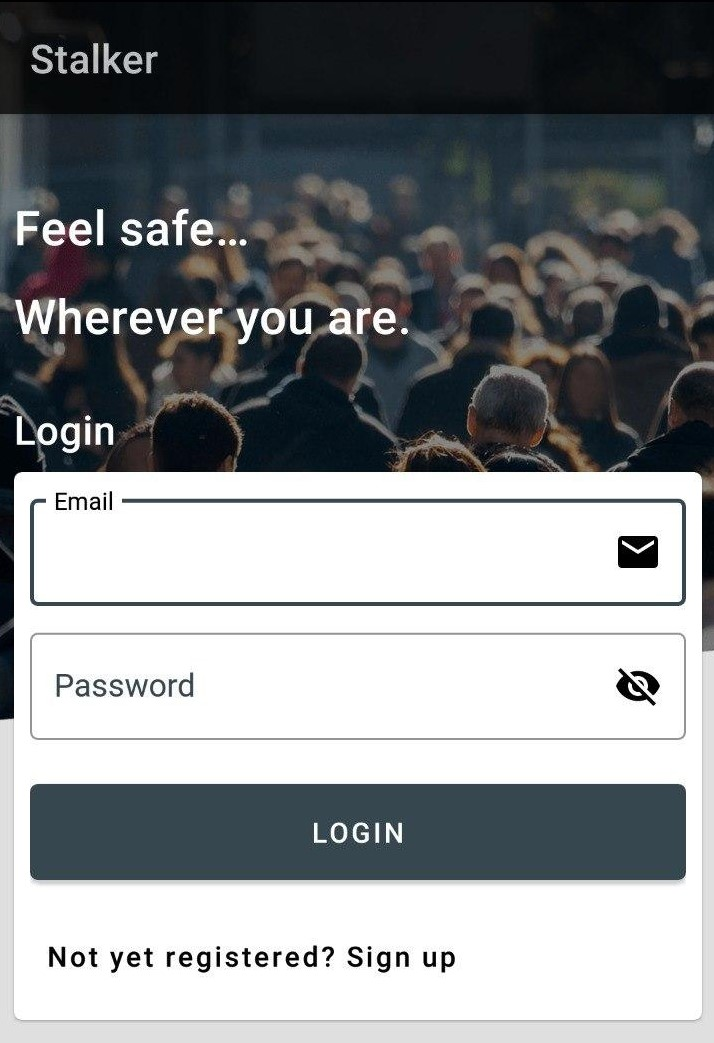
\includegraphics[width=70mm]{pagina-di-accesso.jpg}
    \caption{Pagina di accesso}%
    \label{fig:mobile_app_pagina_di_accesso}
\end{figure}
Al primo avvio di Stalker app, l'utente visualizza la pagina di login.
Per accedere al servizio, l'utente dovrà seguire i seguenti passaggi:
\begin{itemize}
    \item inserire correttamente l'email.
    \item inserire la password. La password può essere visualizzata normalmente durante la sua digitazione, cliccando sull'occhio barrato alla fine del campo d'inserimento.
    \item selezionare il pulsante \textbf{LOGIN} per inviare le credenziali al server.
\end{itemize}
Se i dati inseriti sono corretti, allora l'utente è autorizzato ad entrare in Stalker e cominciare ad essere monitorato (sotto-sezione §~\ref{subs:pagina_organizzazioni}), altrimenti l'accesso a Stalker sarà negato.
Le cause possono essere le seguenti:
\begin{itemize}
    \item l'email inserita non rispetta i vincoli imposti dal sistema di Stalker.
    \item la password non rispetta i vincoli imposti dal sistema di Stalker.
    \item l'email e la password inserite non rispettano i vincoli imposti dal sistema di Stalker.
    \item l'email e la password inserite rispettano i vincoli, ma non sono presenti all'interno del database di Stalker.
\end{itemize}
In ogni caso, il messaggio di errore non sarà specifico ma generico, per motivi di sicurezza.

\subsubsection{Pagina di registrazione}%
\label{subs:pagina_di_registrazione}

\begin{figure}[H]
    \centering
    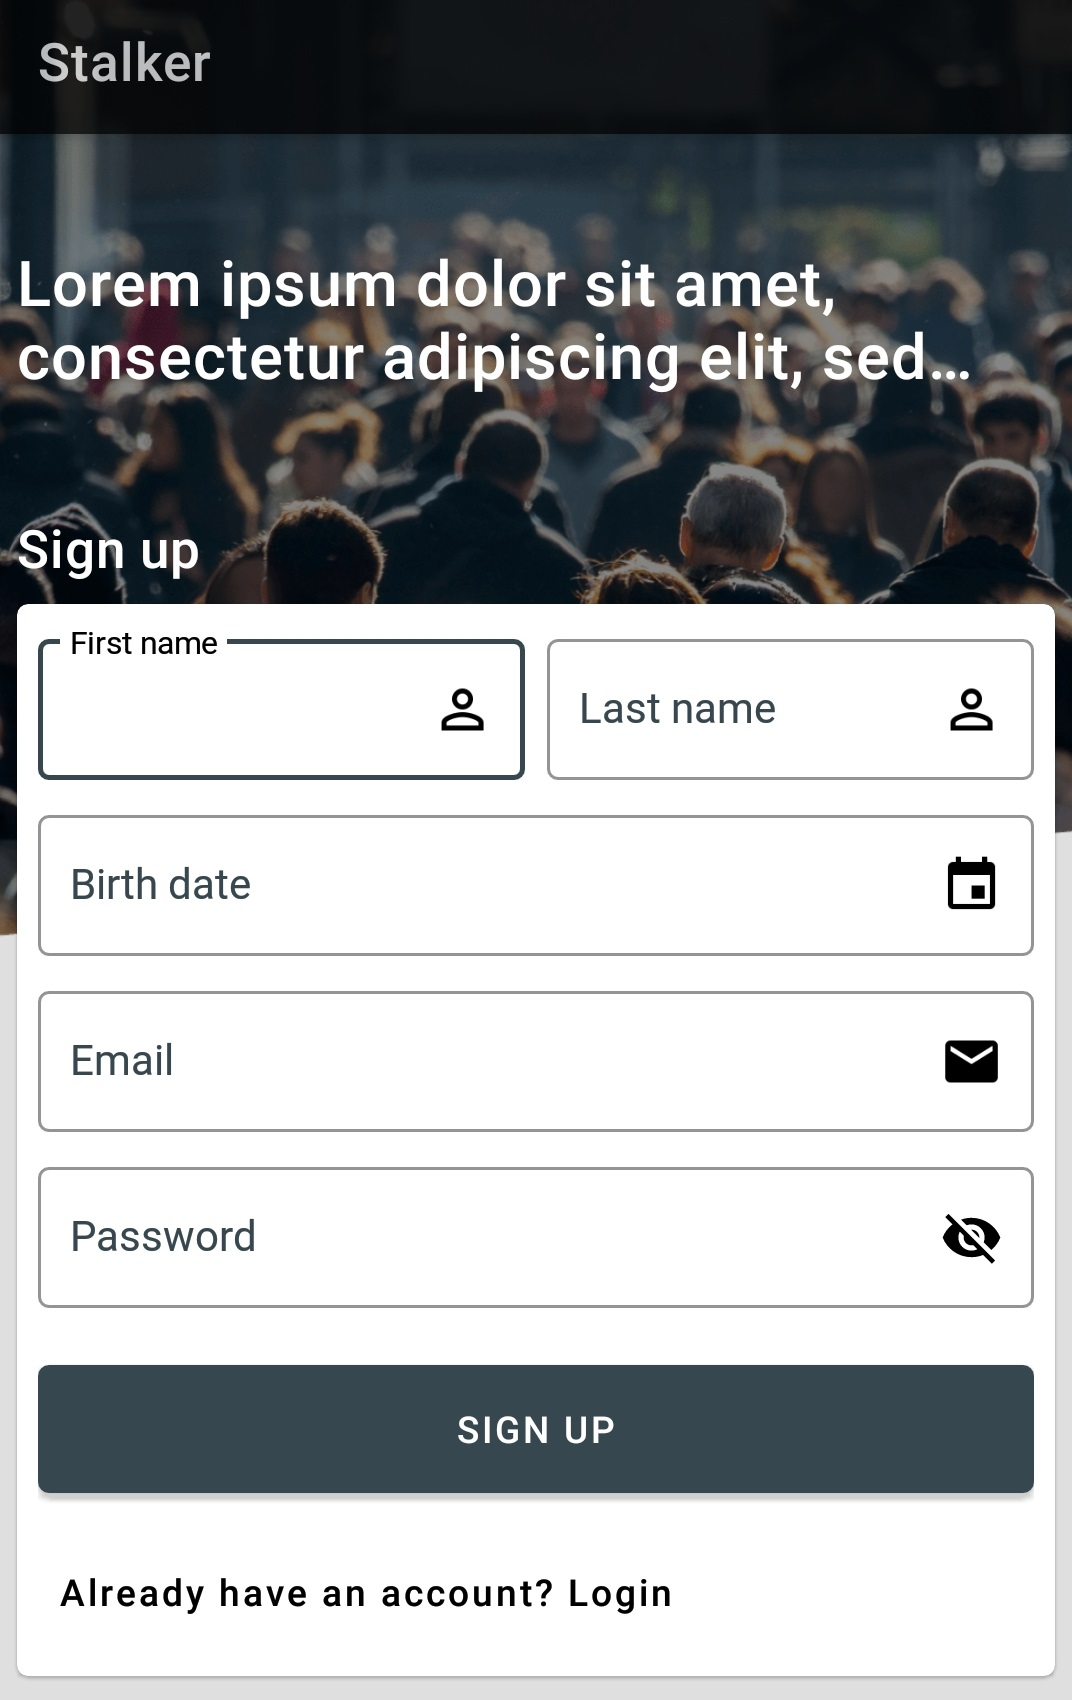
\includegraphics[width=70mm]{pagina-di-registrazione.jpg}
    \caption{Pagina di registrazione}%
    \label{fig:mobile_app_pagina_di_registrazione}
\end{figure}
Se l'utente non possiede delle credenziali di accesso, ha la possibilità di registrarsi, grazie all'apposito form disponibile dopo aver cliccato su \textit{Not yet registered? Sign up}. Per farlo dovrà inserire queste informazioni personali:
\begin{itemize}
    \item il nome.
    \item il cognome.
    \item la data di nascita, che deve essere conforme al formato \textit{yyyy-mm-dd}.
    \item l'email, non già utilizzata in Stalker.
    \item la password che deve contenere almeno 8 caratteri (almeno una lettera maiuscola, una lettera minuscola, un numero ed un simbolo) e al massimo ne può contenere 32. La password può essere visualizzata normalmente durante la sua digitazione, cliccando sull'occhio barrato alla fine del campo d'inserimento.
    \item premere il pulsante \textbf{SIGN UP} per completare la procedura di registrazione.
\end{itemize}
Se i dati inseriti sono corretti, allora l'utente è registrato in Stalker e ha la possibilità di autenticarsi.
In caso contrario, l'utente non è registrato, in quanto la procedura è fallita.
Le cause possono essere le seguenti:
\begin{itemize}
    \item l'email inserita non rispetta i vincoli imposti dal sistema di Stalker.
    \item la password non rispetta i vincoli imposti dal sistema di Stalker.
    \item l'email inserita è già presente nel database.
    \item la data non rispetta il formato \textit{yyyy-mm-dd}.
    \item almeno uno dei campi del form di registrazione non è stato compilato. Sono tutti richiesti.
\end{itemize}
Se l'utente è già in possesso delle credenziali e vuole accedere a Stalker, può raggiungere l'apposito form di autenticazione disponibile cliccando \textbf{Already have an account? Login} (figura §~\ref{fig:mobile_app_pagina_di_accesso}).

\subsubsection{Pagina organizzazioni}%
\label{subs:pagina_organizzazioni}

\begin{figure}[H]
    \centering
    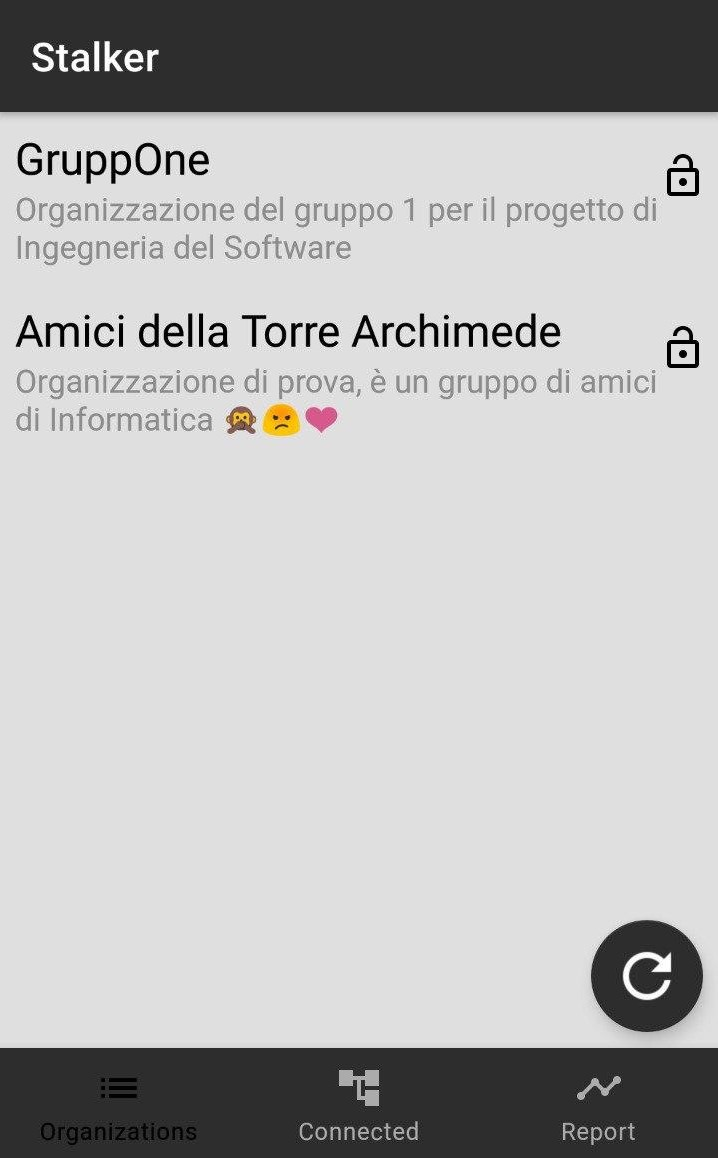
\includegraphics[width=70mm]{pagina-organizzazioni.jpg}
    \caption{Pagina organizzazioni}%
    \label{fig:mobile_app_pagina_organizzazioni}
\end{figure}
Una volta che si è autenticato in Stalker, l'utente visualizza di default una pagina contenente la lista di tutte le organizzazioni registrate in Stalker alle quali si può connettere.
Le informazioni che visualizza per ogni organizzazione sono:
\begin{itemize}
  \item il nome.
  \item la descrizione.
  \item lo stato, ovvero se è pubblica o privata, indicato dal lucchetto che è posto nel bordo destro di ogni singola voce. Il lucchetto aperto indica che l'organizzazione è pubblica, mentre il lucchetto chiuso indica che l'organizzazione è privata e necessita delle credenziali d'accesso specifiche.
\end{itemize}
La pagina offre inoltre due possibili azioni:
\begin{itemize}
  \item aggiornare la lista delle organizzazioni registrate in Stalker, mediante l'apposito pulsante con una freccia ricorsiva che si trova in basso a destra.
  \item cambiare schermata tramite la \glossarioLocale{action bar} posta orizzontalmente in basso nella schermata. La action bar è composta da tre voci:
  \begin{description}
    \item[Organizations:] è la schermata corrente.
    \item[Connected:] l'utente visualizza la lista di organizzazioni alla quale è collegato attualmente (sotto-sezione §~\ref{subs:pagina_organizzazioni_connesse}).
    \item[Report:] l'utente visualizza una serie di dati personali per ogni organizzazione alla quale si è collegato precedentemente (sotto-sezione §~\ref{subs:pagina_report_utente}).
  \end{description}
\end{itemize}
Se l'utente vuole connettersi ad un'organizzazione, può fare \glossarioLocale{tap} su una singola voce dell'elenco.
 \begin{figure}[H]
   \centering
   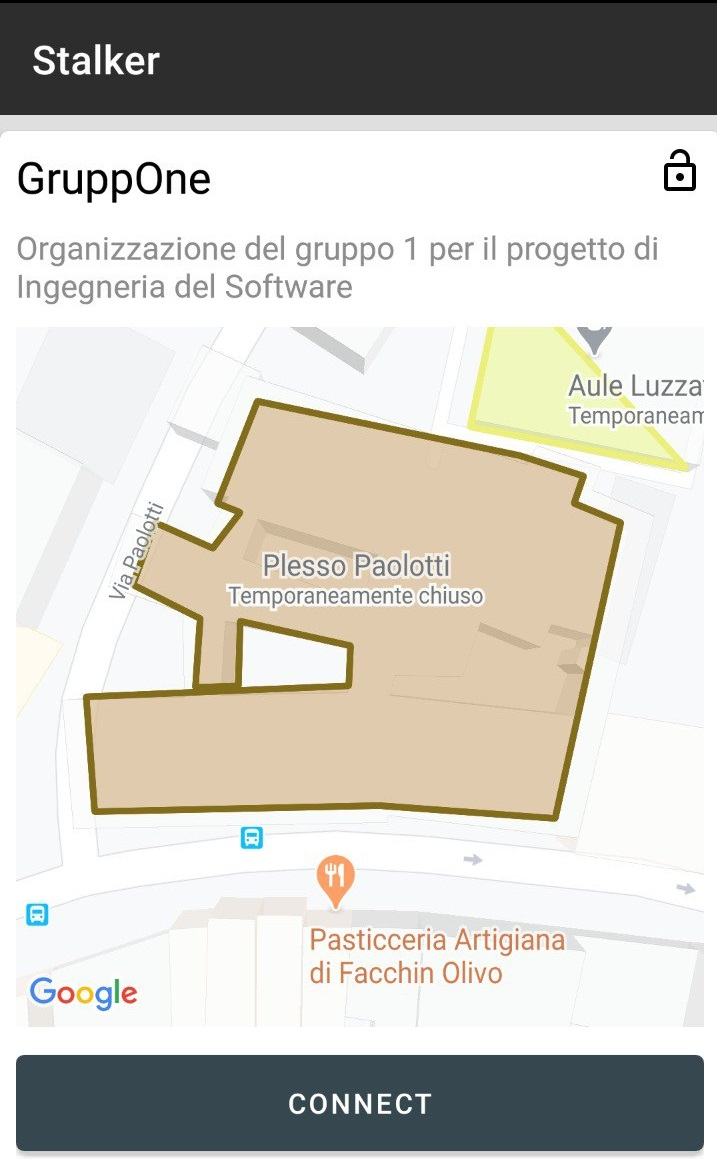
\includegraphics[width=70mm]{selezionamentoorganizzazionepubblica.jpg}
   \caption{Selezionamento organizzazione pubblica}%
   \label{fig:mobile_app_selezionamento_organizzazione_pubblica}
 \end{figure}
Se l'organizzazione selezionata è pubblica, l'utente accede in modo libero senza alcun tipo di restrizione.
% \begin{figure}[H]
%   \centering
%   \includegraphics[width=70mm]{selezionamento-organizzazione-pubblica.jpg}
%   \caption{Selezionamento organizzazione pubblica}%
%   \label{fig:mobile_app_selezionamento_organizzazione_pubblica}
% \end{figure}
Se l'organizzazione selezionata è privata, l'utente deve inserire le credenziali per l'autenticazione \glossarioLocale{LDAP} che corrispondono a:
\begin{description}
  \item[CommonName (CN)]: parte del DomainName (DN) che si riferisce ad uno specifico utente.
  \item[Password]: la password LDAP dell'utente per accedere all'organizzazione privata.
\end{description}
Se l'utente inserisce le credenziali in modo errato, l'accesso all'organizzazione non è consentita.
Nel caso in cui la connessione all'organizzazione, pubblica o privata che sia, va a buon fine, l'utente viene indirizzato ad una schermata con tutte le informazioni relative ad essa.


\begin{figure}[H]
  \centering
  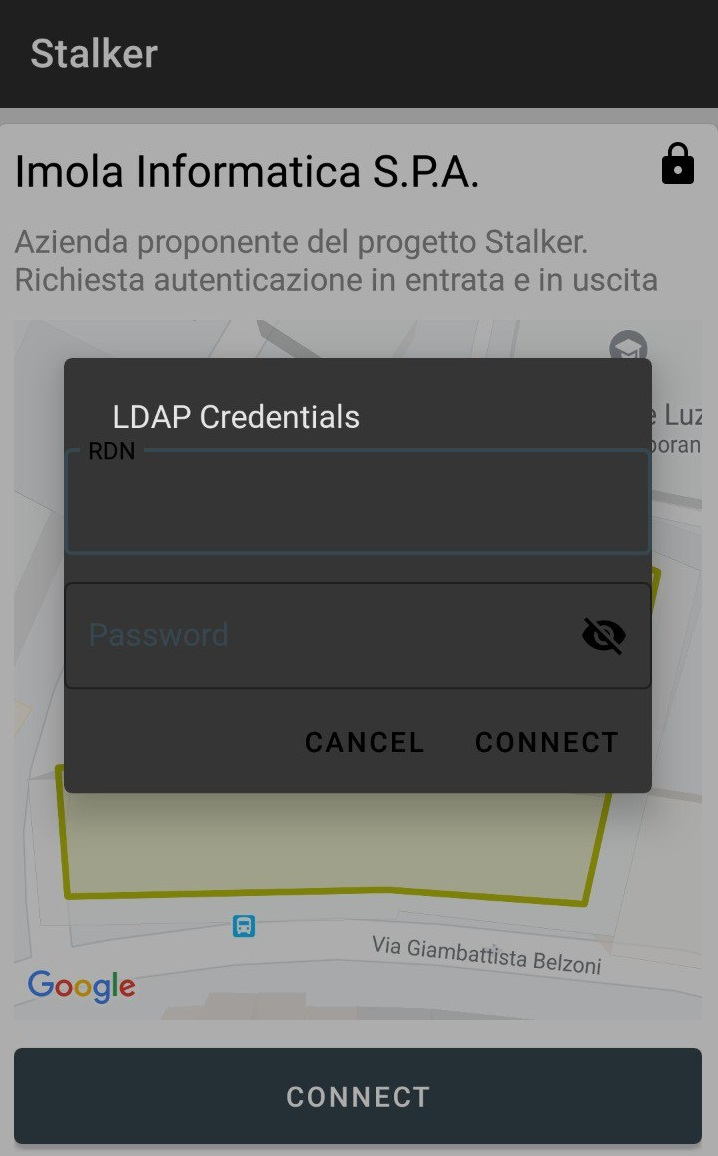
\includegraphics[width=70mm]{collegamentoldap.jpg}
  \caption{Pagina di collegamento}%
  \label{fig:mobile_app_pagina_collegamento_ldap}
\end{figure}

% Le informazioni dell'organizzazione che vengono visualizzate sono: %TODO
% \begin{itemize}
%   \item
% \end{itemize}

%TODO
\subsubsection{Pagina organizzazioni connesse}%
\label{subs:pagina_organizzazioni_connesse}

 \begin{figure}[H]
   \centering
   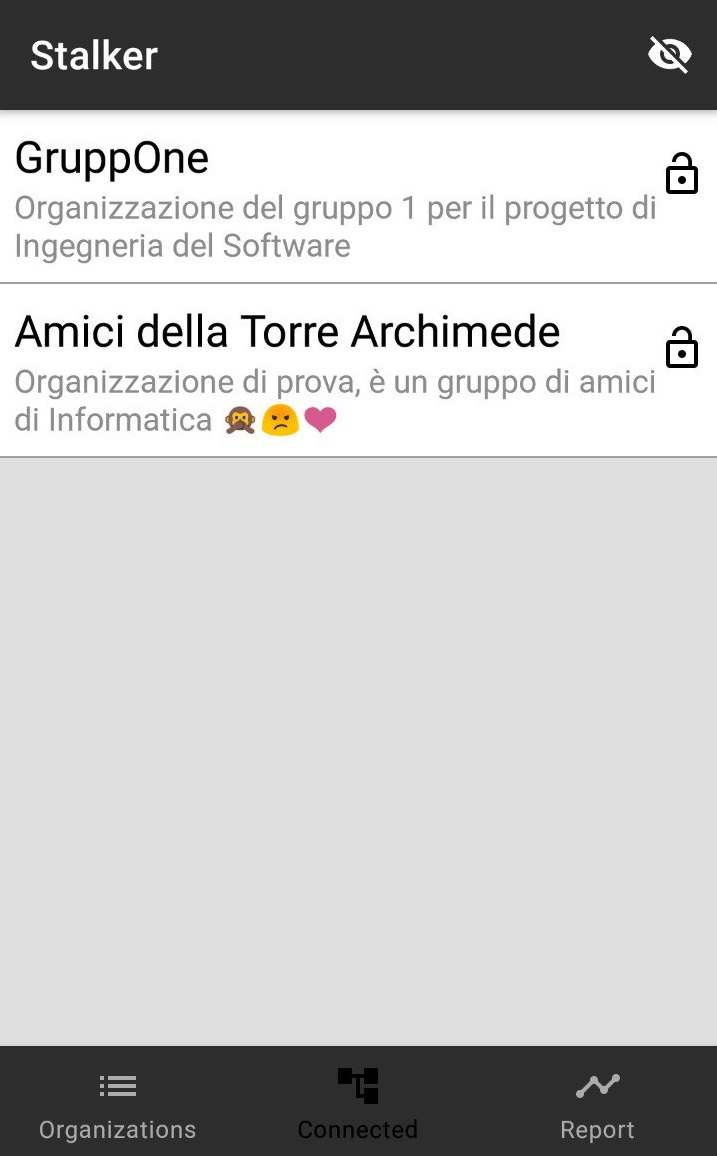
\includegraphics[width=70mm]{paginaconnesse.jpg}
   \caption{Pagina organizzazioni connesse}%
   \label{fig:mobile_app_pagina_organizzazioni_connesse}
 \end{figure}

 Una volta che l'utente si collega ad una o più organizzazioni visualizza di default una pagina contenente la lista di tutte le organizzazioni a cui è collegato in Stalker e alla quale si può disconnettere.
 Le informazioni che visualizza per ogni organizzazione sono:
 \begin{itemize}
   \item il nome.
   \item la descrizione.
   \item lo stato, ovvero se è pubblica o privata, indicato dal lucchetto che è posto nel bordo destro di ogni singola voce. Il lucchetto aperto indica che l'organizzazione è pubblica, mentre il lucchetto chiuso indica che l'organizzazione è privata e necessita delle credenziali d'accesso specifiche.
 \end{itemize}
 La pagina offre due possibili azioni:
 \begin{itemize}
   \item cambiare il proprio stato da noto ad incognito o da incognito a noto tramite l'icona apposita in alto a destra.
   \item cambiare schermata tramite la action bar posta orizzontalmente in basso nella schermata. La action bar è composta da tre voci:
   \begin{description}
     \item[Organizations:] l'utente visualizza la lista di organizzazione alla quale non è collegato e si può collegare (sotto-sezione §~\ref{subs:pagina_organizzazioni}).
     \item[Connected:] è la schermata corrente.
     \item[Report:] l'utente visualizza una serie di dati personali per ogni organizzazione alla quale si è collegato precedentemente (sotto-sezione §~\ref{subs:pagina_report_utente}).
   \end{description}
 \end{itemize}
 Se l'utente vuole disconnettersi da un'organizzazione, può fare tap su una singola voce dell'elenco.

\subsubsection{Pagina report utente}%
\label{subs:pagina_report_utente}

 \begin{figure}[H]
   \centering
   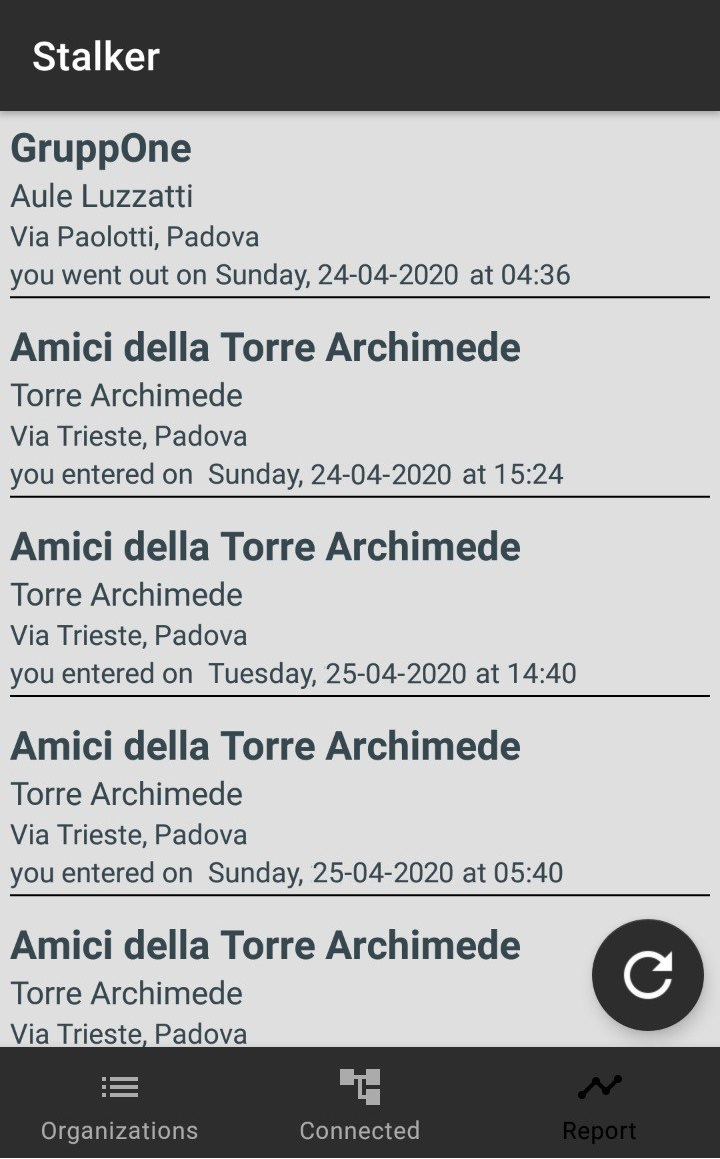
\includegraphics[width=70mm]{paginareportutente.jpg}
   \caption{Pagina report utente}%
   \label{fig:mobile_app_pagina_report_utente}
 \end{figure}

Una volta che l'utente si è autenticato può visualizzare una pagina contenente un report di tutti gli accessi effettuati in una o più organizzazioni.
Le informazioni visualizzate nella pagina per ogni organizzazione sono:
\begin{itemize}
    \item il nome.
    \item il luogo.
    \item l'indirizzo del luogo.
    \item la data e l'ora di accesso all'organizzazione.
\end{itemize}
La pagina offre inoltre due possibili azioni:
\begin{itemize}
  \item aggiornare la lista delle organizzazioni del report, mediante l'apposito pulsante con una freccia ricorsiva che si trova in basso a destra.
  \item cambiare schermata tramite la action bar posta orizzontalmente in basso nella schermata. La action bar è composta da tre voci:
  \begin{description}
    \item[Organizations:] l'utente visualizza la lista di organizzazione alla quale non è collegato e si può collegare (sotto-sezione §~\ref{subs:pagina_organizzazioni}).
    \item[Connected:] l'utente visualizza la lista di organizzazioni alla quale è collegato attualmente (sotto-sezione §~\ref{subs:pagina_organizzazioni_connesse}).
    \item[Report:] è la schermata corrente.
  \end{description}
\end{itemize}



\subsection{Risoluzione dei problemi}%
\label{subs:mobile_app_risoluzione_problemi}

\subsubsection{Attivazione sorgenti sconosciute}%
\label{subs:mobile_app_attivare_sorgenti_sconosciute}

L'applicazione Stalker viene scaricata da una sorgente che è ritenuta \textit{sconosciuta} dal sistema operativo Android, in quanto il link dalla quale viene scaricata non è una fonte verificabile e ritenuta sicura rispetto al \textit{Play Store}, che è il negozio ufficiale delle applicazioni Android.
GruppOne vuole evidenziare fin da subito che Stalker non ha fini malevoli che mirano a danneggiare la sicurezza dell'utente e che l'applicazione mobile non è presente nel \textit{Play Store} per motivazioni economiche, prese in accordo con tutti i componenti del team.
A fronte di questa premessa, l'utente vuole installare l'applicazione mobile Stalker, ma viene allertato con questo messaggio:
\textbf{Installazione bloccata:} \textit{Per motivi di sicurezza, il telefono è impostato per bloccare l'installazione di applicazioni ottenute da fonti sconosciute.}
L'utente quindi deve autorizzare il sistema operativo Android ad installare Stalker, in quanto sorgente sconosciuta. La procedura è la seguente:
\begin{itemize}
    \item accedere alle impostazioni.
    \item cercare la dicitura \textit{Origini sconosciute} o \textit{Sorgenti sconosciute}.
    \item attivare l'impostazione facendo tap su di esso.
    \item è possibile che il vostro sistema operativo Android vi chieda se attivare questa impostazione \textbf{solo} per questa applicazione. Per motivi di sicurezza, vi consigliamo di rispondere in modo affermativo.
\end{itemize}
Ora che è stata attivata questa impostazione, è possibile tornare alla finestra precedente e proseguire la procedura di installazione.

\subsubsection{Errore durante l'installazione}%
\label{subs:mobile_app_errore_installazione}

Nel caso \textit{Stalker} non si installi nel dispositivo in modo corretto, preghiamo l'utente di verificare i requisiti descritti nella sezione §~\ref{sub:mobile_app_requisiti}.
Se il problema dovesse persistere anche in caso di requisiti soddisfatti, vi preghiamo di segnalarcelo nelle modalità discusse nella sezione §~\ref{sec:supporto_tecnico}.

\subsubsection{Accesso all'applicazione non disponibile}%
\label{subs:mobile_app_accesso_non_disponibile}

Nel caso ci fossero problemi con il collegamento all'applicazione mobile, vi consigliamo di controllare se è attiva una rete Internet nel vostro smartphone Android.
Nel caso in cui la rete sia abilitata vi preghiamo di riprovare l'accesso in un secondo momento.
Se il problema dovesse persistere, vi preghiamo di segnalarlo nelle modalità discusse nella sezione §~\ref{sec:supporto_tecnico}.

\subsubsection{Errore nel reperimento della posizione}%
\label{subs:mobile_app_errore_posizione}

Nel caso il vostro smartphone non riuscisse a reperire la vostra posizione, vi consigliamo di verificare se è attiva la geolocalizzazione (GPS) nel vostro smartphone Android.
Se la geolocalizzazione dovesse essere attiva, vi consigliamo di provare a seguire i seguenti passaggi:
\begin{itemize}
    \item Accedere alle impostazioni del vostro smartphone, tramite l'apposita icona oppure tramite la tendina delle notifiche.
    \item Accedere alla sezione \textit{Applicazioni} oppure \textit{App e notifiche}. Nel caso questa sezione abbia un altro nome, vi consigliamo di consultare il manuale del vostro smartphone e ricercare la pagina rilevante le applicazioni installate.
    \item Cercare l'applicazione \textit{Stalker} tra quelle nella lista e selezionarla.
    \item Accedere alla sezione \textit{Autorizzazioni} o \textit{Permessi} e verificare se i permessi riguardante la geolocalizzazione sono attivi.
    \item Nel caso non fossero attivi, attivare la geolocalizzazione per \textit{Stalker}.
\end{itemize}
Nel caso i passi indicati non siano risultati utili ai fini del funzionamento di \textit{Stalker}, verificare il corretto funzionamento della geolocalizzazione attraverso altre applicazioni.
Se il problema è di natura tecnica, vi preghiamo di contattare il vostro \textit{\glossarioLocale{vendor}} al più presto.
Se il problema persiste solamente in \textit{Stalker}, vi preghiamo di segnalarlo nelle modalità discusse nella sezione §~\ref{sec:supporto_tecnico}.

\end{document}
